% Introducción

\chapter{Segmentación de tumores}

\section{Descripción del dataset}

\href{https://www.kaggle.com/datasets/pkdarabi/brain-tumor-image-dataset-semantic-segmentation} {Link} del dataset. 

Este dataset contiene 2146 imágenes con sus respectivas máscaras y está subdivivido en conjuntos de entrenamiento (1502 archivos), validación (429 archivos) y test (215).

 En la Fig. \ref{fig.mask} se observa la superposición de una imagen del dataset con su respectiva máscara, indicando la ubicación del tumor.
 
 
\begin{figure}[H]
\centering
        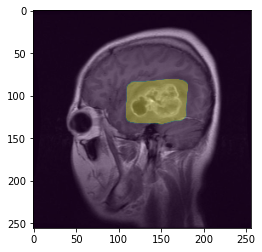
\includegraphics[width=0.3\linewidth]{chapters/segmentacion/images/mask.png}
        \caption{Imagen junto con la máscara indicando el tumor.}
        \label{fig.mask}
  \end{figure}


\section{Preprocesamiento de las imágenes}

Las imágenes disponibles tenían todas el mismo tamaño $(640\times640)$. Con el objetivo de normalizar las imágenes, se optó por redimensionarlas a una resolución de ($256 \times 256$) píxeles. 

Se aplicó una conversión a escala de grises, dado que esta representación es ampliamente utilizada en el ámbito del diagnóstico médico, garantizando así una compatibilidad estándar para el análisis y la interpretación de las imágenes.

Un último preprocesamiento que se aplicó es normalizar el rango de valores de los píxeles de la imagen, originalmente cada píxel $p_{ij}\in [0,255]$ y luego de la transformación $p_{ij}\in [0,1]$.

Las máscaras eran imágenes binarias del mismo tamaño que la imagen sobre la que segmenta. 


\section{Modelo: UNET}

Como modelo de segmentación se utilizó la red ampliamente utilizada UNET, cuya arquitectura se muestra en la Fig. \ref{fig.unet}. 

\begin{figure}[H]
\centering
        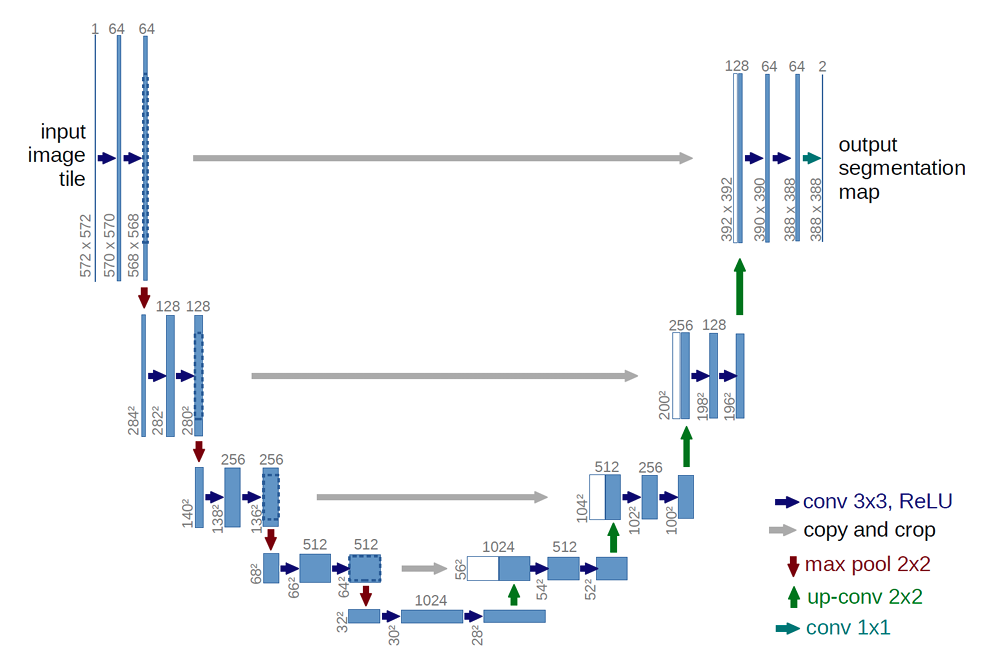
\includegraphics[width=0.7\linewidth]{chapters/segmentacion/images/unet.png}
        \caption{UNET}
        \label{fig.unet}
  \end{figure}

Esta arquitectura consta de un bloque de cuatro encoders, un bloque convolucional y un bloque de cuatro decoders. 

El optimizador utilizado fue $\textit{adam}$, la función de pérdida $\textit{dice loss}$ tomando como métrica $\textit{dice coefficient}$. Se entrenó la red con un $\textit{batch size}$ de 10, $\textit{validation split}$ de 0.2 y con 100 $\textit{epochs}$. Se implementó un callback de EarlyStopping. 

Dado que el target de este modelo es una máscara, una imagen, tenía más sentido tomar como función de pérdida el coeficiente de Dice, el cual se define como:

\begin{equation}
DSC(X,Y) = \frac{2|X\cap Y|}{|X|+|Y|}
\end{equation}.

Este coeficiente es igual a 1 si y solo si $X=Y$, y 0 si $X$ e $Y$ son no conexos. Esto codifica matemáticamente la superposición de la máscara obtenida con la máscara target. 

Antes de calcular las métricas correspondientes de clasificación para este modelo, se procedió a investigar si hubo un overfitting durante el entrenamiento. Para esto se graficó la función de pérdida y el accuracy tanto de train como de test para cada epoch. La gráfica se muestra en la Fig. \ref{fig.loss}. 


\begin{figure}[H]
\centering
        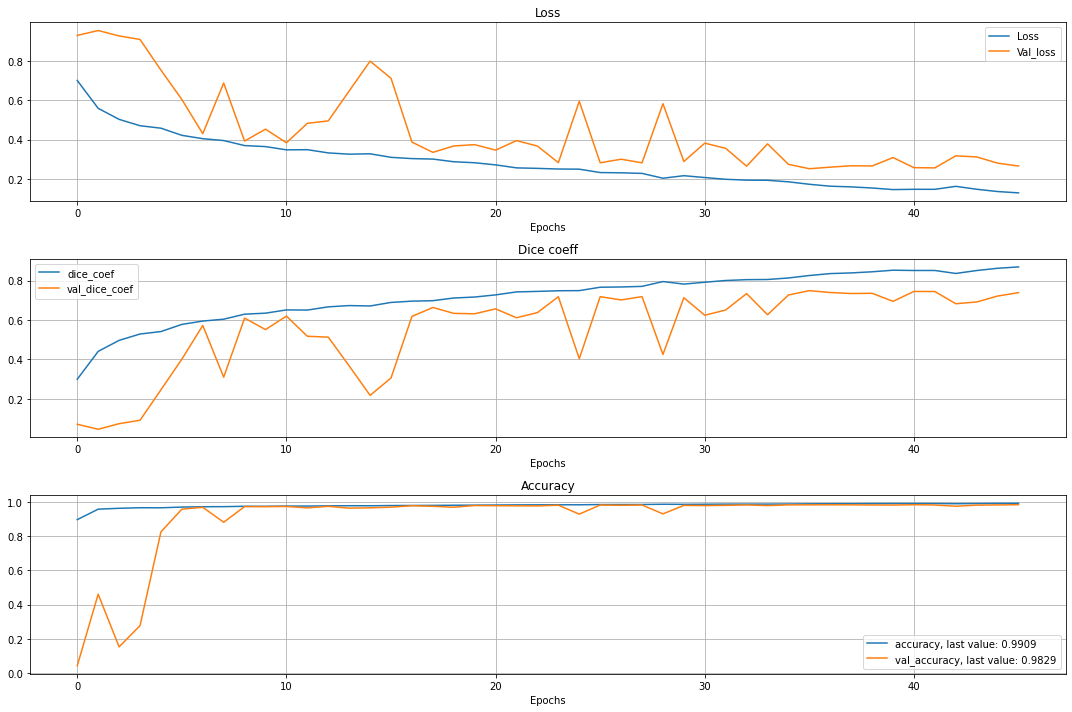
\includegraphics[width=0.8\linewidth]{chapters/segmentacion/images/metricas.png}
        \caption{Función de pérdidas y accuracy para la red UNET.}
        \label{fig.loss}
  \end{figure}

Observando las gráficas anteriores se observa que el modelo no overfitea. 

A continuación se procedió a calcular las métricas correspondientes. En este caso se calculó el coeficiente de Dice para cada conjunto de datos, los cuales se muestran en la Fig. \ref{fig.dice}.


\begin{figure}[H]
\centering
        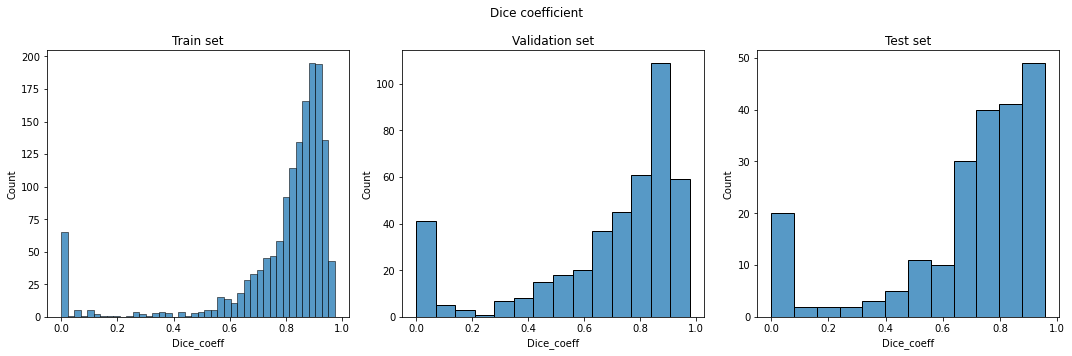
\includegraphics[width=0.9\linewidth]{chapters/segmentacion/images/dice.png}
        \caption{Coeficiente de Dice para cada conjunto de imágenes.}
        \label{fig.dice}
  \end{figure}

Se observa que en todos los casos, el valor máximo de la distribución está cercano a uno, indicando que el modelo funcionó razonablemente bien. Es notable observar que existen algunos coeficientes menores que uno. Esto se explica considerando que las máscaras usadas como target eran perfectamente rectangulares, mientras que las máscaras predichas por el modelo no lo son, sino que intentan adaptarse al tumor copiando su forma, como se observa en la Fig. \ref{fig.mascaras}. 

\begin{figure}[H]
    \centering
    \begin{subfigure}[b]{0.4\textwidth}
        \centering
        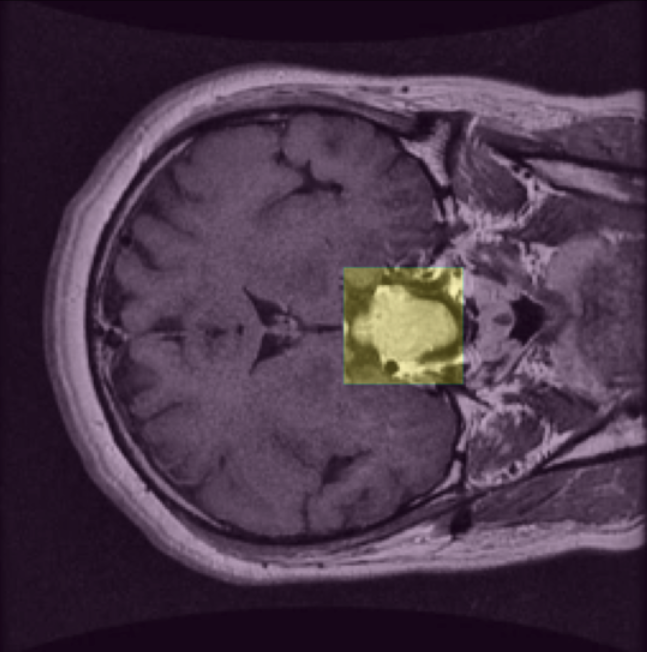
\includegraphics[width=\textwidth]{chapters/segmentacion/images/mask_train.png}
        \caption{Máscara target}
        \label{fig:imagen1}
    \end{subfigure}
    \hfill
    \begin{subfigure}[b]{0.4\textwidth}
        \centering
        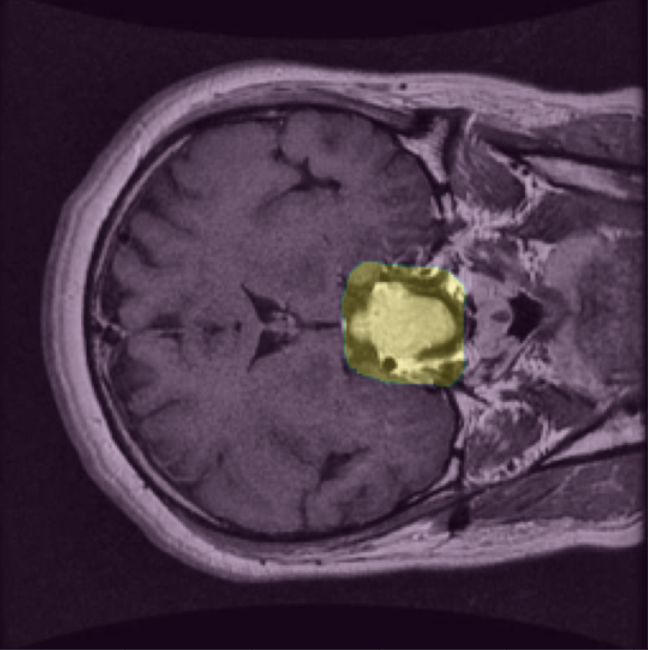
\includegraphics[width=\textwidth]{chapters/segmentacion/images/mask_pred.png}
        \caption{Máscara predicha}
        \label{fig:imagen2}
    \end{subfigure}
    \caption{Diferencias entre máscaras}
    \label{fig.mascaras}
\end{figure}

En el código subido a Github está el detalle de los cálculos realizados, así como un slider para poder ver las imágenes con sus correspondientes máscaras.












